%%%%%%%%%%%class file
\documentclass[12pt]{article}




%this command gives the journal no. 
%
%\jno{dnnxxx}
%%%%%%%%%%%%%%


%%%%%%%%%%%%%%%%%
%call  packages
%\usepackage{natbib}
%%%%%%%%%%%%%%

%%%%%%%%%%%%%%%%%%

\usepackage{amsmath,amsthm,bm,mathrsfs}
\usepackage{graphicx}
\usepackage{placeins}
\usepackage{caption}
\usepackage{floatrow}
\usepackage[utf8]{inputenc}
\usepackage[T1]{fontenc}
\usepackage{lmodern}
\usepackage{apacite}

%%%%%%%%%%%%%%%%%


%%%%%%%%%%%
%this files contains Theorem styles based in IMA JOURNALS
%
\input standard.tex

%%%%%%%%%%%%%


\renewcommand{\theequation}{\thesection.\arabic{equation}}
\numberwithin{equation}{section}
\def\citeasnoun{\cite}
\usepackage[utf8]{inputenc}
\usepackage{hyperref}



\begin{document}

%%%%%%%%%%%%%%%%%
\title{Análisis evolutivo de insectos transgénicos de la especie \textit{Rhodnius prolixus} en el tratamiento de la enfermedad de Chagas}
\author{ {\sc Sergio Hernández Charpak y Nancy Ruiz Uribe}\\[2pt]
Biología Sintética. Departamento de Física. Universidad de los Andes \\[6pt]
{\rm [Fecha de entrega: Mayo 22 de 2015]}\vspace*{6pt}}
\maketitle

%%%%%%%%%%%%%%%%%abstract style
%Two grouping braces are necessary in abstract environment
%first argument contains abstract text; second argument contains keywords
%text

%%%%%%%%%%%%%%%%%%%%%%%%%%%%%%%



%%%%%%%%%%%%%%section A%%%%%%%%%
\section{Introducción}

La enfermedad de Chagas o Tripanosomiasis americana es una enfermedad parasitaria tropical causada por el parásito protozoario \textit{Trypanosoma cruzi}. Afecta a mamíferos y humanos y es transmitida por un insecto triatomino del género \textit{Rhodnius prolixus}.Ataca el sistema nervioso, el sistema digestivo y el corazón y hoy en día mueren 50 000 personas al año debido a esta enfermedad (Bonney, 2014). Dado que no existe por el momento una cura o una vacuna definitiva contra esta enfermedad, se hace necesaria la búsqueda de nuevos mecanismos de ataque contra la reproducción y diseminación del parásito. Uno de los mecanismos de prevención es la erradicación de los triatominos, sin embargo, esto es una tarea díficil debido a las consecuencias ecológicas.  
La biología sintética es un campo en desarrollo que brinda herramientas con prometedores resultados. Siendo el parásito \textit{Trypanosoma cruzi} el agente etiológico de la enfermedad de Chagas, se piensa que si se logra inhibir su crecimiento dentro los vectores de propagación, se podría disminuir la acción de la enfermedad. Esto se quiere lograr con la inserción de un plásmido pRrMDWK6 dentro de 3 tipos de bacterias simbiontes diferentes: Escherichia coli, Rhodococcus rhodnii y Salmonella. La acción de este plásmido vendrá dada por la codificación de un gen VHK que producirá el fragmento de un anticuerpo llamado rDB3, que se unirá a la progesterona presente en la superficie del parásito, inhibiendo de esta forma su crecimiento y reproducción dentro del intestino del insecto. \\
Se quiere realizar un análisis evolutivo de la inserción del plásmido en las 3 bacterias previamente mencionadas para conocer cuál de estas bacterias presenta un mejor fitness o adaptación al plásmido y por ende una mejor difusión de anticuerpo dentro del intestino del vector y una mejor erradicación del parásito.
La transformación de bacterias para impedir el crecimiento del parásito dentro del insecto ha sido efectuado previamente y se ha confirmado su éxito. Esto ha sido posible gracias al uso de plásmidos o elementos integrativos de ADN, péptidos tripanocidas (como Cecropin A) y fragmentos de anticuerpos de cadena simple. (Beard et al., 2001)
Debido a que los insectos se alimentan únicamente de sangre a lo largo de su desarrollo, su dieta es deficiente en algunas vitaminas y minerales. Es por esto que los insectos mantienen una relación de simbiosis con la bacteria \textit{R.rhodnii} y \textit{E.coli}. \textit{Salmonella} aún no ha sido testeada para simbiosis pero es una potencial candidata.(Mandrioli, 2009) \\

Para llevar acabo la paratransgénesis es necesario que una población de microbios, de vectores y de parásitos esté disponible en el laboratorio, así como los métodos para aislar y transformar la bacteria simbionte. Así mismo, para que el método funcione adecuadamente, la transformación de las bacterias simbiontes debe resultar en mutantes estables, sin pérdida de fitness reproductivo. Los mutantes deberían tener una tasa de crecimiento similar a los no-mutantes, de tal forma que al liberarlos al ambiente no resulte en una competencia por selección natural que termine erradicando los vectores transformados.\\
Es por esto que es de nuestro interés realizar un modelo evolutivo que nos permita encontrar entre 3 bacterias diferentes cuál de ellas resulta teniendo una mejor adaptación a la transformación y de esta forma optimizar el proceso de paratránsgenesis.\\

Para ello será necesario medir de manera experimental el fitness de cada una de las bacterias con y sin la inserción del plásmido. Debido a que realizar esto en clase no fue posible, fue necesario buscar y encontrar constantes que se asemejaran a una posible función de fitness de cada una de nuestras bacterias. Con la ayuda del modelo de Moran fue posible simular un escenario evolutivo de una población total de 90 vectores para cada una las bacterias, y con ayuda del algoritmo de Guillespie se simuló la cantidad de bacterias producidas dentro de cada vector luego de la transformación. A continuación se muestra el diseño experimental, el modelo evolutivo, las consideraciones éticas y las dificultades generales de nuestro proyecto.


\begin{figure}[!ht]
\begin {center}
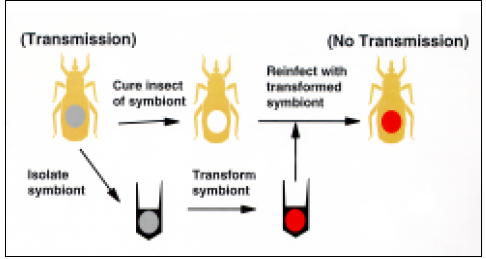
\includegraphics[width=0.4\textwidth]{conversion.PNG}
\caption{Idea general de la paratránsgenesis}
\end {center}
\FloatBarrier
\end{figure}


\section{Protocolo y diseño experimental}

\subsection{Cultivo y transformación de las bacterias}

Las bacterias R.rhodnii, E.coli y Salmonella serán crecidas un medio Luria-Bertani que contenga el antibiótico kanamicina. 


\subsection{Construcción del plásmido pRrMDWK6}

La expresión y secreción del anticuerpo rDB3 es controlada por un gen derivado del bacilo \textit{Mycobacterium kansasii} (Mk$\alpha$). El protocolo para la extracción de este gen está disponible en Matsuo et al., 1990. Mk$\alpha$ será amplificado usando los siguientes primers de la reacción en cadena de la polimerasa (PCR): \textbf{5'-GC TCT AGA GTT AAC TAT TCT TTG TAC GCG-3'}(sentido 5'-3') y \textbf{5'-GC GAA CGC TCC CGC GGT CGC-3'}(sentido 3'-5'). El 1er primer será incorporado al sitio de restricción de la enzima Xba1 5' y el 2ndo primer será incorporado al sitio de restricción de la enzima Sac II. El gen que condificará para el anticuerpo DB3 será amplificado utilizando los siguientes primers: \textbf{5'-GC ACC GCG GGA GCC CAG GTG AAA CTG CTC-3'} (sentido 5'-3') y \textbf{5'-CCT CGA TTG CGG CCG CTT AAC-3'}(sentido 3'-5'). El 1er primer se incluirá en un sitio SacII donde será posible ligarlo con la secuencia Mk$\alpha$. El fragmento reverso será clonado en el fragmento XbaI. El complejo Mk$\alpha$DB3Vh/K será clonado en un sitio XbaI del plásmido. Se clonará también un gen de resistencia a la kanamicina como un fragmento  Bam HI y de esta forma se construirá el plásmido final. En la siguiente imagen es posible ver el plásmido con todas las enzimas de los restricción y los diferentes genes. (Durvasula et al., 1999)

\begin{figure}[!ht]
\begin {center}
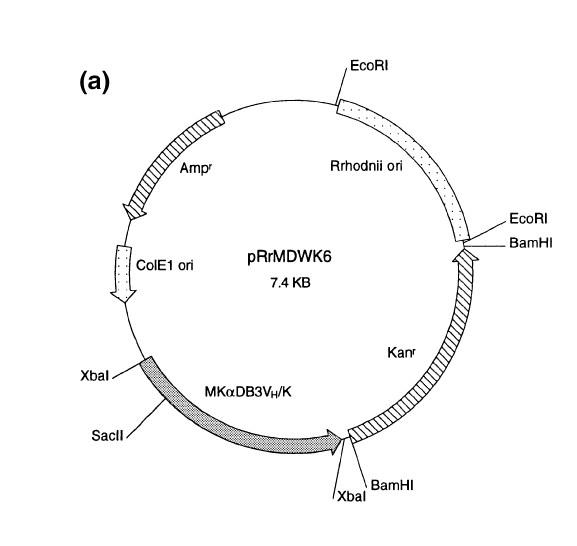
\includegraphics[width=0.4\textwidth]{plasmido+.PNG}
\caption{Plásmido de inserción. Origen de replicación de R.rhodnii: Rhodnii ori; Kan: gen de resistencia de kanamicina, cassete de secreción y expresión de MKaDB3VH/K, rDB3; Origen de replicación para E.coli: ColE1 ori, gen de resistencia: Ampicilina. (Durvasula et al., 1999)}
\end {center}
\FloatBarrier
\end{figure}

\begin{figure}[!ht]
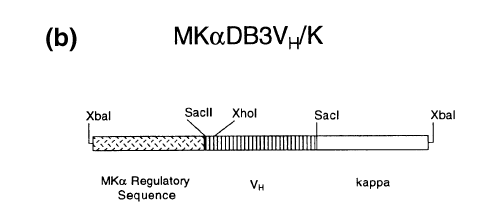
\includegraphics[width=0.4\textwidth]{cassete.PNG}
\caption{Cassete de expresión y secreción MKaDB3VH/K, rDB3. (Durvasula et al., 1999)}
\FloatBarrier
\end{figure}

El objetivo de usar el promotor y el peptido de señal de \textit{Mycobacterium kansasii} es el de producir el fragmento de un anticuerpo de cadena libre (rDB3) que se unirá posteriormente a la progesterona presente en la superficie corporal del parásito \textit{Trypanosoma cruzi} y de esa forma inhibir su crecimiento. Varios estudios demuestran que el fragmento del anticuerpo puede ser expresado y no será degradado en el tracto digestivo del parásito y permanece funcional. (Beard et al., 2001)\\
rDB3 es un anticuerpo murino monoclonal cuya función es la adherirse a la progesterona con una afinidad de $(K\sim 10^9 M^-1)$. Este anticuerpo ha podido producirse sin problema en \textit{E.coli} y \textit{R.rhodnii} (He et al., 1995). Sin embargo es necesario confirmar la producción del mismo en el espacio periplásmico de \textit{Salmonella}.\\
Pese a que los insectos tienen alguna capacidad de reconocer anticuerpos externos a ellos, su sistema de detección no es tan sofisticado como el de los mamíferos. Así que la producción de un anticuerpo que no les pertenece a ellos no genera necesariamente una respuesta del sistema imune del individuo, permitiendo así que el gen se exprese libremente.\\


\subsection{Transformación de los vectores}
Colonias de \textit{R.prolixus} serán mantenidas a 26 grados y a una humedad relativa de 75$\%$ en un insectario, si el experimento se decide hacer en el campus universitario, los insectos podrían ser solicitados al CIMPAT. Se tomarán dos grupos de 45 individuos cada uno, el primer grupo será de control y en este se insertarán bacterias que no tengan el plásmido o que no estén geneticamente modificadas mientras que en el otro grupo se insertarán las bacterias que codifican para la producción del anticuerpo.(Durvasula et al., 1999). Los vectores de control tendrán una sepa de bacteria que no exhiba resistencia a la kanamicina. Los vectores serán  alimentados con sangre infectada durante períodos de 1 mes y en cada etapa de desarrollo se tomarán 9 insectos de cada uno de los grupos y se tomará el contenido de sus intenstinos para realizar el conteo de bacterias y de parásitos.
De la misma forma después de cada de alimentación sanguínea se contará el número de vectores que sobreviven con cada una de las bacterias transformadas.

\subsubsection{Introducción de las bacterias en los vectores}

Los simbiontes pueden ser introducidos en \textit{R.prolixus} mediante alimentación con sangre.Las bacterias que crecen en medio pueden ser añadidas a sangre de conejo que después puede ser proveída a los insectos por medio de un aparato para alimentación especial, o bien, por medio de cropofagia (Beard et al., 2001)

\subsubsection{Genes marcadores:}
El gen de resistencia de kanamicina (kanamycin resistance gene) es usado para marcar los vectores genéticamente modificados en presencia del antibiótico kanamicina y es eficiente al matar los vectores que no lo están. La ventaja de este gen es que puede ser usado tanto en \textit{R.rhodnii} como en \textit{E.coli} (Beard et al., 2001) Al final de cada generación de insectos se tendrá el número de colonias de bacterias y de vectores que sobrevivieron a la ingesta de sangre contaminada con \textit{T.cruzi} con la ayuda del marcador.

\subsection{Reconocimiento del anticuerpo por medio de la técnica de Western Blot}
La técnica de Western Blot (o Inmunoblot) es ampliamente usada para reconocer proteínas en una muestra de tejido. Se usa la electroforesis en geles de poliacrilamida para separar proteínas nativas en su estructura terciaria o ya denaturadas. Para saber si después de la transformación los insectos modificados están produciendo el anticuerpo rDB3, se tomará una muestra del tejido del intenstino y se analizará la presencia del anticuerpo por medio de esta técnica. Para el Western Blot se usará 1 $\mu$g de proteína y se usará una solución diluida de 1:1000 partes de fosfatasa alcalina conjugada con un anticuerpo igG para reconocer el anticuerpo rDB3. (Durvasula et al., 1999).
Se utilizará un marcador de peso molecular similar al peso del anticuerpo rDB3 para confirmar mediante electroforesis en gel de poliacrilamida si se está produciendo efectivamente el anticuerpo. Se espera obtener algo de la siguiente forma:

\begin{figure}[!ht]
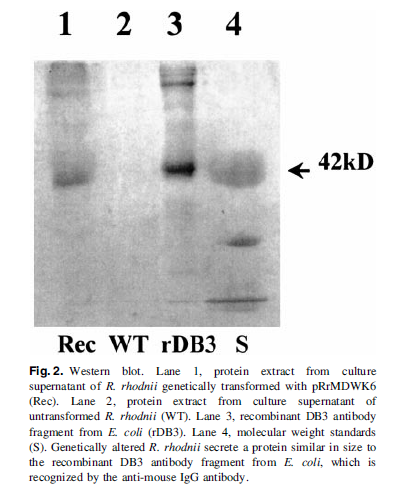
\includegraphics[width=0.4\textwidth]{electrof.PNG}
\caption{Electroforesis en gel de poliacrilamida. Reconocimiento del anticuerpo rDB3}
\FloatBarrier
\end{figure}


\subsection{Test para simbiosis de la bacteria \textit{Salmonella}}
Se ha encontrado información relevante sobre la simbiosis de \textit{R.rhodnii} y \textit{E.coli} (Dionisio et al., 2005). Sin embargo es necesario confirmar si la bacteria Salmonella es un simbionte adecuado para R.prolixus. Para confirmar esto se pueden realizar experimentos en los que se infectan los vectores con la bacteria y mirar si la población de vectores disminuye o crece de manera significativa.


\section{Modelo evolutivo}
\subsection{Escogencia de las constantes}


Nuestro modelo evolutivo consiste en comparar las poblaciones de vectores sobrevivientes genéticamente modificados con las 3 diferentes bacterias para al final concluir cuál de las bacterias es más eficiente a la hora de producir el anticuerpo necesario para reducir las poblaciones de \textit{T.cruzi}. Sin embargo, es necesario realizar varios experimentos en los que se pueda medir el fitness de las bacterias de manera precisa. Después de una intensa búsqueda sólo fue posible encontrar los fitness de \textit{E.coli} y \textit{Salmonella} en presencia de plásmidos. En el artículo de Dionisio et al., (2005) se efectuaron varios experimentos en los que se medía el fitness de bacterias de \textit{E.coli} en presencia y ausencia del plásmido R1. El valor para el fitness escogido fue de 2.051$\pm$0.087. \\
Para la bacteria \textit{Salmonella} se encontró la siguiente información obtenida de Dionisio et al., (2005): "We observed that the Salmonella cells bearing the evolved plasmid have a significantly higher fitness (1.558$\pm$0.059, nZ3) than Salmonella cells without the R1 plasmid (1.000$\pm$0.074, nZ3; two-tailed t-test, p-value Z=0.007)." Gracias a esta información fue posible para nosotros cuantificar en iPython mediante el algoritmo de Guillespie de la tarea 3 el número de vectores que se producen a lo largo de un lapso de un tiempo según sus fitness.
Para la bacteria R.rhodnii no ha sido posible encontrar fitness con o sin plásmido. Sin embargo, ha sido posible encontrar el numero de colonias sobrevivientes después de varias de generaciones, con o sin el plásmido, dentro de los vectores R. prolixus. Esta información fue obtenida de Durvasula et al., (1999), se tiene para las ninfas de 2nda, 3era, 4ta y 5ta generación y para los adultos, un total de colonias resistentes a la kanamicina de 1.19, 5.95, 14.4, 40.1 y 457.6  colonias respectivamente con sus respectivas incertidumbres. Se puede observar que a medida que aumentan las generaciones también aumenta el número de colonias significativamente, por lo cual se puede inferir que el fitness es mayor a 1. El valor que hemos escogido de manera aleatoria teniendo en cuenta el orden de magnitud de este tipo de constantes es de 1.2.

\subsection{Algoritmo de Guillespie para modelar el crecimiento poblacional de bacterias}

El algoritmo de Gillepsie se utilizó para realizar un primer acercamiento a modelar el crecimiento poblacional de bacterias. El modelo al ser simplista, no aporta mucha más información que los datos de entrada (los fitness). 

El código implementado en IPython se puede observar en \url{http://nbviewer.ipython.org/github/sercharpak/Biologia_Sintetica_Proyecto/blob/master/IPython/Modelo_Evolutivo_1.0.ipynb}.\\

A continuación podemos observar los resultados obtenidos para 100 corridas con $ 10^{5}$ puntos cada una.\\

\begin{figure}[!ht]
\begin{floatrow}
\ffigbox{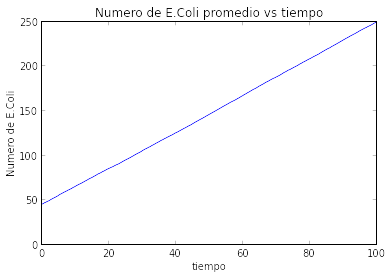
\includegraphics[scale = 0.45]{ecoli_lineal.png}}{\caption{Crecimiento de E.Coli}\label{ecoli_lineal}}
\ffigbox{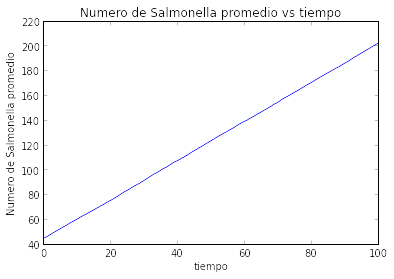
\includegraphics[scale = 0.45]{salmonella_lineal.png}}{\caption{Crecimiento de Salmonella}\label{salmonella_lineal}}
\end{floatrow}
\FloatBarrier
\end{figure}

\begin{figure}[!ht]
\begin{floatrow}
\ffigbox{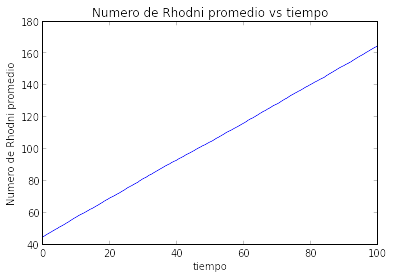
\includegraphics[scale = 0.45]{rhodnii_lineal.png}}{\caption{Crecimiento de E.Coli}\label{rhodnii_lineal}}
\ffigbox{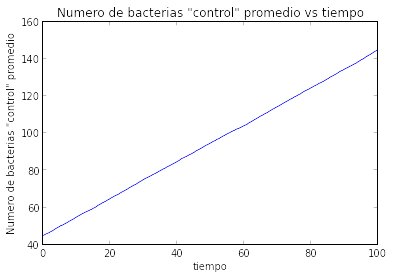
\includegraphics[scale = 0.45]{control_lineal.png}}{\caption{Crecimiento con fitness de 1}\label{control_lineal}}
\end{floatrow}
\FloatBarrier
\end{figure}
\FloatBarrier
Podemos observar un comportamiento netamente lineal. No se llega a un estado estable ya que no hay ninguna restricción.\\

Se puede observar a continuación como los crecimientos se encuentran en el mismo orden que los fitness utilizados. De mayor a menor, E.coli, Salmonella, R.Rhodnii, y el control con fitness de 1.\\
\begin{figure}[!ht]
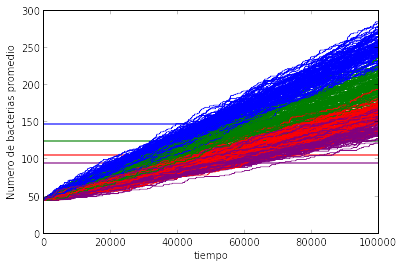
\includegraphics[width=0.7\textwidth]{todasLasCorridas.png}
\caption{Diferentes crecimientos para las diferentes bacterias}
\FloatBarrier
\end{figure}
\FloatBarrier
Los ruidos obtenidos crecen exponencialmente, pero luego se estabilizan todos alrededor del mismo valor $0.07-0.08$.\\

\begin{figure}[!ht]
\begin{floatrow}
\ffigbox{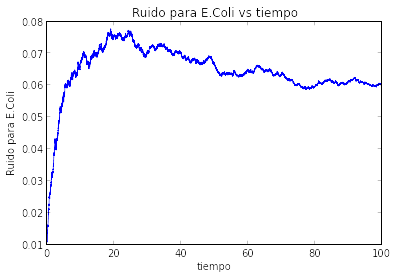
\includegraphics[scale = 0.45]{ruido_ecoli.png}}{\caption{Ruido de E.Coli}\label{ruido_ecoli}}
\ffigbox{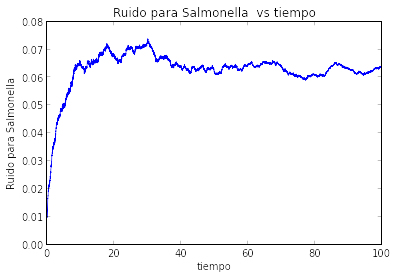
\includegraphics[scale = 0.45]{ruido_salmonella.png}}{\caption{Ruido de Salmonella}\label{ruido_salmonella}}
\end{floatrow}
\FloatBarrier
\end{figure}
\FloatBarrier

\begin{figure}[!ht]
\begin{floatrow}
\ffigbox{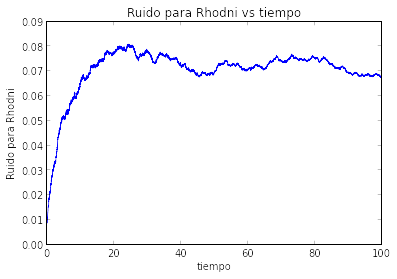
\includegraphics[scale = 0.45]{ruido_rhodnii.png}}{\caption{Ruido de R.Rhodnii}\label{ruido_rhodnii}}
\ffigbox{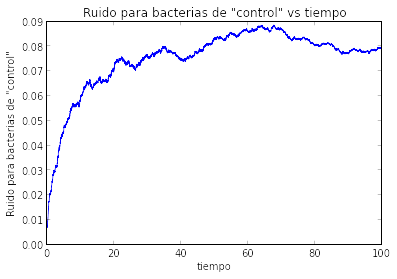
\includegraphics[scale = 0.45]{ruido_control.png}}{\caption{Ruido del control con fitness de 1}\label{ruido_control}}
\end{floatrow}
\FloatBarrier
\end{figure}
\FloatBarrier
Y las distribuciones para el último estado para cada una de las bacterias son igualmente muy similares. Parecen corresponder a grandes rasgos a una distribución gausiana.\\

\begin{figure}[!ht]
\begin{floatrow}
\ffigbox{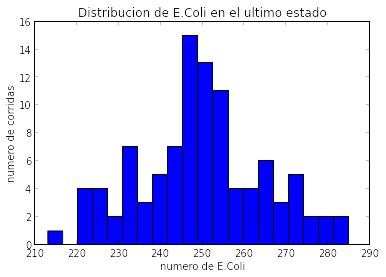
\includegraphics[scale = 0.45]{distri_ecoli.png}}{\caption{Distribución de E.Coli para el último estado}\label{distri_ecoli}}
\ffigbox{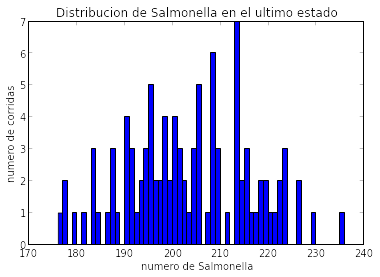
\includegraphics[scale = 0.45]{distri_salmonella.png}}{\caption{Distribución de Salmonella para el último estado}\label{distri_salmonella}}
\end{floatrow}
\FloatBarrier
\end{figure}
\FloatBarrier

\begin{figure}[!ht]
\begin{floatrow}
\ffigbox{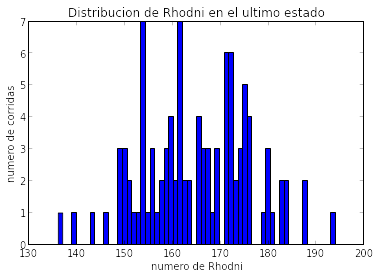
\includegraphics[scale = 0.45]{distri_rhodnii.png}}{\caption{Distribución de R.Rhodnii para el último estado}\label{distri_rhodnii}}
\ffigbox{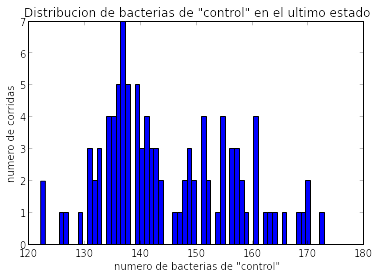
\includegraphics[scale = 0.45]{distri_contr.png}}{\caption{Distribución de control con fitness de 1 para el último estado}\label{distri_contr}}
\end{floatrow}
\FloatBarrier
\end{figure}
\FloatBarrier

\subsection{Modelo de Moran para simular evolución bajo fitness relativo}

El proceso de Moran es un proceso de muerte-nacimiento que describe selección natural en poblaciones finitas. Para una población de tamaño N, en este caso 90, la población se divide en dos tipos: población transformada (A) y población no transformada (B). El número de individuos de A con i y el número de los individuos de B se denota por N-i. Se denota como $f_A$ y $f_B$ los fitness de cada una de las poblaciones.(Harper,2013)\\
Se describen así las siguientes probabilidades de transición para el crecimiento, disminución y el estancamiento:
\[ T_{i \rightarrow i+1}= \frac{i f_{A} \left(i\right) \left( 1 - \mu_{AB} \left(i\right) \right) + \left( N-i \right) f_{B} \left(i\right) \mu_{BA} \left(N-i\right) }{i f_{A}\left(i\right)+ \left(N-i\right) f_{B}\left(i\right)} \frac{N-i}{N}\]
\[ T_{i \rightarrow i-1}= \frac{i f_{A} \left(i\right) \mu_{AB} \left(i\right) + \left( N-i \right) f_{B} \left(i\right)\left(1- \mu_{BA} \left(N-i\right) \right) }{i f_{A}\left(i\right)+ \left(N-i\right) f_{B}\left(i\right)} \frac{i}{N}\]
\[ T_{i \rightarrow i}= 1 - T_{i \rightarrow i+1} - T_{i \rightarrow i-1} \]

Con $\mu_{AB}$ y $\mu_{BA}$ las probabilidades de mutación que dependerán del estado, entre otras cosas.

El repositorio que contiene todo el código implementado en Mathematica se puede acceder en \url{https://github.com/sercharpak/Biologia_Sintetica_Proyecto}. Por simplicidad se implementó un modelo de fitness relativo (A con fitness dado y B con fitness de 1). A continuación se muestran las imágenes obtenidas después de graficar una población total de N=90 vectores con cada una de las bacterias.\\
Para E.coli se tiene:\\

\begin{figure}[!ht]
\begin{floatrow}
\ffigbox{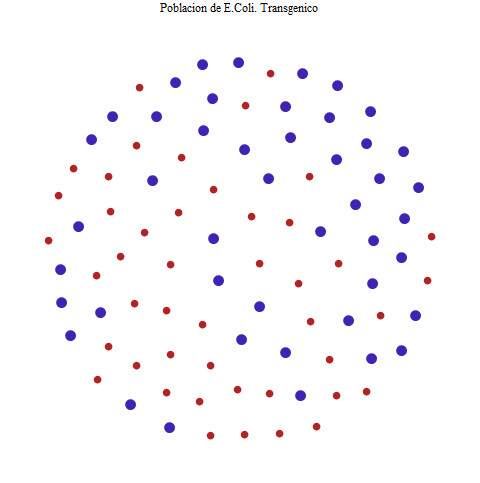
\includegraphics[scale = 0.3]{ecoli_moran_1.png}}{\caption{Generación $\#$0. Rojo= Población B. Azul= Población A}\label{ecoli_1}}
\ffigbox{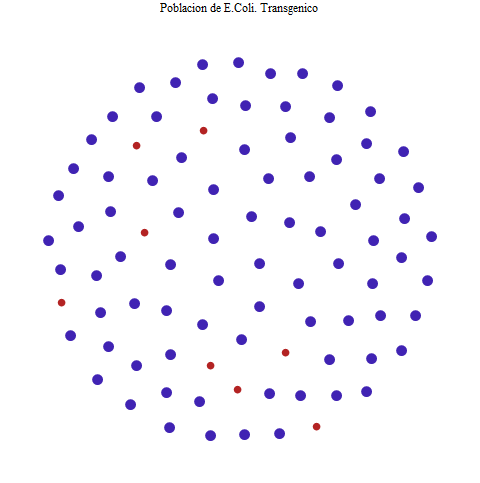
\includegraphics[scale = 0.3]{ecoli_moran_339.png}}{\caption{Generación $\#$339. Rojo= Población B. Azul= Población A}\label{ecoli_339}}
\end{floatrow}
\FloatBarrier
\end{figure}
\FloatBarrier        

\begin{figure}[!ht]
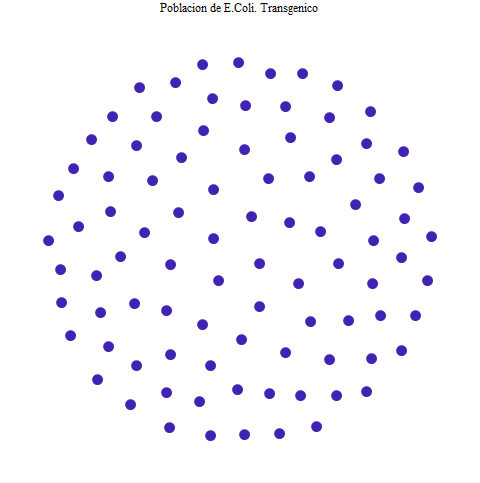
\includegraphics[width=0.35\textwidth]{ecoli_moran_576.png}
\caption{Generación $\#$576. Rojo= Población B. Azul= Población A }
\FloatBarrier
\end{figure}
\FloatBarrier
\ Se puede observar que a medida que pasan las generaciones va dominando la población de color azul, es decir, las bacterias transformadas con el plásmido. Esto se debe a que el fitness de estas últimas es mayor al fitness de las bacterias sin transformar.\\

Para R.rhodnii:\\

\begin{figure}[!ht]
\begin{floatrow}
\ffigbox{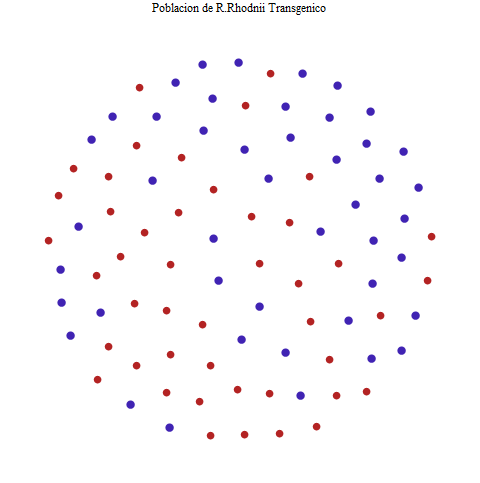
\includegraphics[scale = 0.35]{rhodnii_moran_1.png}}{\caption{Generación $\#$0. Rojo= Población B. Azul= Población A}\label{rhod_1}}
\ffigbox{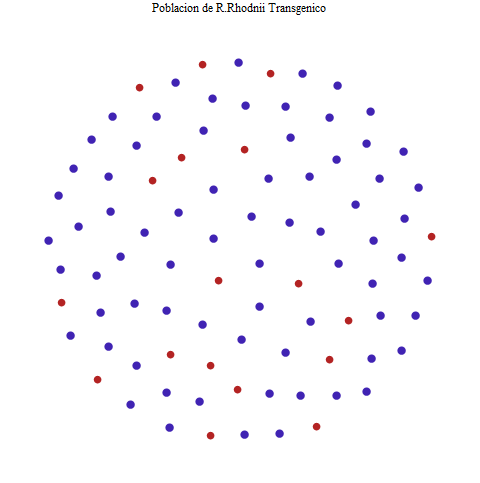
\includegraphics[scale = 0.35]{rhodnii_moran_477.png}}{\caption{Generación $\#$477. Rojo= Población B. Azul= Población A}\label{rhod_477}}
\end{floatrow}
\FloatBarrier
\end{figure}
\FloatBarrier

\begin{figure}[!ht]
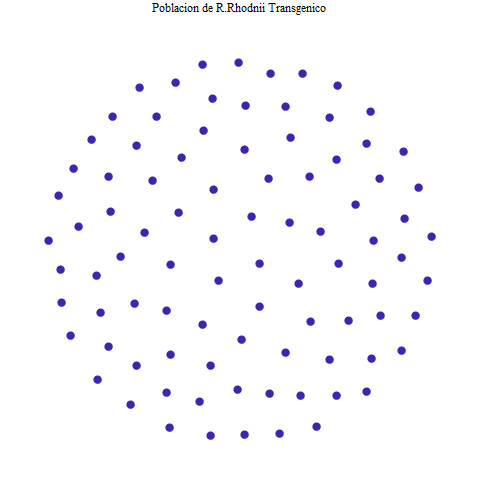
\includegraphics[width=0.35\textwidth]{rhodnii_moran_947.png}
\caption{Generación $\#$947. Rojo= Población B. Azul= Población A }
\FloatBarrier
\end{figure}
\FloatBarrier
Se puede realizar la misma observación con \textit{R.Rhodnii}. Sin embargo se puede observar que el número de generaciones necesarias para que toda la población sea de un mismo tipo es mucho mayor (casi el doble).\\

Para Salmonella:\\

\begin{figure}[!ht]
\begin{floatrow}
\ffigbox{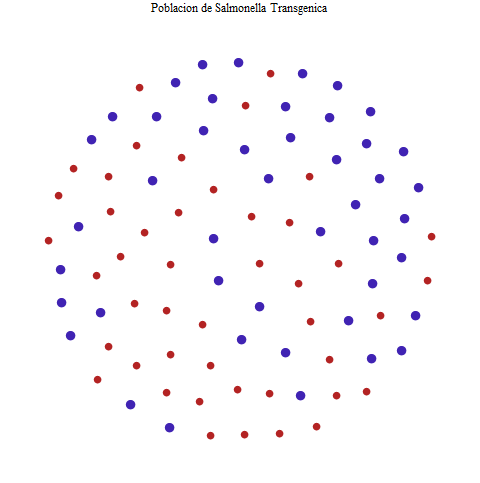
\includegraphics[scale = 0.35]{samonella_moran_1.png}}{\caption{Generación $\#$0. Rojo= Población B. Azul= Población A}\label{salm_1}}
\ffigbox{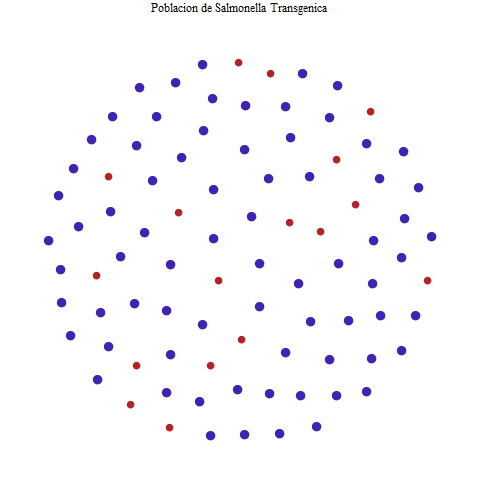
\includegraphics[scale = 0.35]{samonella_moran_496.png}}{\caption{Generación $\#$496. Rojo= Población B. Azul= Población A}\label{salm_496}}
\end{floatrow}
\FloatBarrier
\end{figure}
\FloatBarrier
Se puede observar el mismo comportamiento, y se puede notar que el número de generaciones necesiarias para que toda la población sea de un mismo tipo se encuentra entre el de \textit{E.Coli} y el de \textit{R.Rhodnii}, al igual que los fitness escogidos.\\

Se obtienen las siguientes gráficas de crecimiento poblacional:\\\\

\begin{figure}[!ht]
\begin{floatrow}
\ffigbox{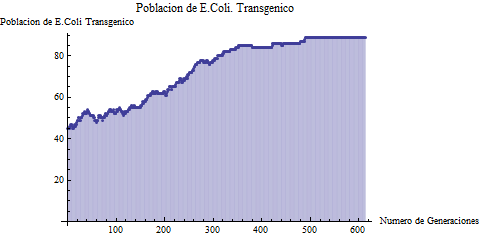
\includegraphics[scale = 0.4]{poblacion_ecoli_trans.png}}{\caption{Población de E.coli transformada}\label{pobl_ecol}}
\ffigbox{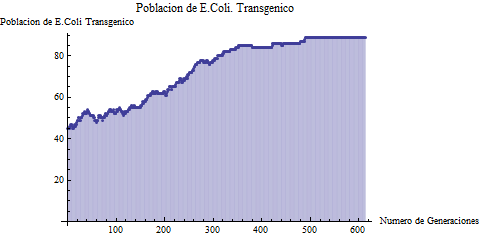
\includegraphics[scale = 0.4]{poblacion_ecoli_trans.png}}{\caption{Población de Salmonella transformada}\label{pobl_salm}}
\end{floatrow}
\FloatBarrier
\end{figure}
\FloatBarrier


\begin{figure}[!ht]
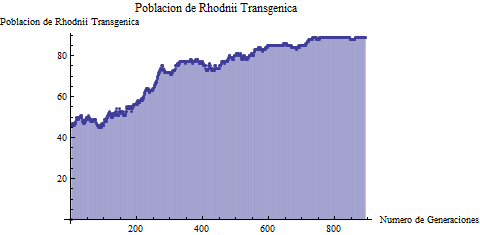
\includegraphics[width=0.5\textwidth]{poblacion_rhodnii_trans.png}
\caption{Población de R.rhodnii transformada}
\FloatBarrier
\end{figure}
\FloatBarrier

\section{Consideraciones éticas}

La manipulación genética de insectos que transmiten enfermedades es una potencial alternativa para la eliminación de enfermedades peligrosas que afectan la salud humana. Productos de expresión de genes insertados que puedan bloquear o eliminar la producción de patógenos dentro de los vectores de transmisión puede ser una herramienta valiosa en el control de estas enfermedades. Sin embargo es necesario tener en cuenta las consecuencias ecólogicas, éticas y ambientales de la introducción de organismos geneticamente modificados en el ambiente.


\subsection{Transferencia horizontal de genes}

La THG es un importante proceso a nivel biólogico que suele darse particularmente en la evolución de las bacterias y es importante en el proceso de resistencia a antibioticos y regulación virulenta. En el libro \textit{Pathogenesis of Leishmaniasis} se generó un modelo matemático que predice la TGH entre una \textit{R.rhodnii} y \textit{G.rubropertincus} genéticamente modificadas. El modelo predice una frecuencia de TGH de menos de $1.14 \times 10^-16$ por 100.000 generaciones a un nivel de certeza del 99$\%$. Esto significa que ls frecuencia de TGH es menor a un estimado de 10$^-1$ por gen por 1000 generaciones. Lo cual sugiere que la probabilidad de que estos eventos ocurran es muy poca. 	


\subsection{Consecuencias ecólogicas y regulación}

Pueden existir varias consecuencias ecólogicas a la hora de liberar organismos genéticamente modificados al ambiente. En particular, si los vectores con bacterias modificadas son liberados y presentan cambios negativos en el fitness, es posible que estos organismos tengan menos posibilidad de sobrevivir y por ende se extingan más fácil dentro de la población, llevando a una disminución significativa de estos triatominos en su ambiente. Esto sin duda conlleva a consecuencias graves en la cadena trófica y ecología de otros animales.\\
Si la liberación de los vectores se realiza en áreas donde habitan humanos, es necesario primero hacer pruebas y experimentos con humanos y esto necesitaría una aprobación especial de la entidad que regula este tipo de trámites.\\
Así mismo, para poder liberar organismos modificados, se necesita el permiso de las autoridades de las comunidades afectadas.\\
La autoridad encargada de regular la investigación y esparcimiento de organismos genéticamente modificados en Colombia aún no existe (veáse Tarea 3).Es posible que este tipo de cuestiones estén relacionadas con el Ministerio de Medio Ambiente o el Instituto Nacional de Salud, pero hasta el momento no se ha encontrado una legislación o proyecto de ley claro que tenga que ver con este tema.


\section{Dificultades generales}

\subsection{Evolución del proyecto}

A lo largo de este proyecto se experimentaron diversas dificultades desde su inicio. El tema escogido es de gran relevancia debido a la gran cantidad de víctimas de la enfermedad de Chagas. Esto nos impulsó a lanzarnos en este tema. En un comienzo se aspiró en estudiar una droga que afecta de manera agresiva a T.Cruzi. \\
Sin embargo, en la \textbf{primera retroalimentación}, se nos informó que era de poco interés para el contexto del curso debido a su costo y su poca viabilidad. El principal consejo era centrarse en los vectores de T.Cruzi e inhibir el crecimiento de este dentro de ellos. Decidimos entonces centrarnos en el anticuerpo Rdb3 que, al atarse a la progesterona, inhibe el crecimiento de T.cruzi dentro de los vectores. En este instante identificamos de manera exitosa los diferentes elementos necesarios para el proyecto.\\ Luego de la \textbf{segunda retroalimentación}, se nos informó que el modelo era demasiado simplista y era mejor hacer un análisis de la difusión de nuestra bacteria y de el anticuerpo rdb3 dentro del vector. \\
En la \textbf{tercera retroalimentación}, caímos en cuenta que nuestro análisis de difusión no tenía aplicación en este caso ya que ambos parásito y bacteria se encuentran en el mismo lugar dentro del vector.
Evolucionamos así al proyecto actual: Análisis evolutivo de bacterias transgénicas para escoger la mejor bacteria entre \textit{R.Rhodnii}, \textit{E.Coli} y \textit{Salmonella Enterica}.\\

\subsection{Constantes}
La búsqueda de constantes y datos en la literatura fue exhausitva. Debido a la necesidad de trabajo experimental para obtener dichas constantes, estas son extremádamente escasas en la literatura. Esto tuvo como consecuencia que se usaran valores de fitness de \textit{E.Coli} y \textit{Salmonella} con otro plásmido, R1 y no pRrMDWK6 y que se estimara un valor para el fitness de \textit{R.Rhodnii} con base a una obvervación de evolución de poblaciones. Por lo tanto utilizar estas constantes aumenta la incertidumbre de nuestro modelo de manera importante.

\subsection{Modelo}
El modelo de evolución población utilizado fue simplificado debido a la falta de conocimiento en el tema de parte nuestra. Por ello se realizó un análisis simplista con base al algoritmo de Gillepsie desarrollado en el curso. Sin embargo el análisis en ambos modelos fue superficial y no se pudieron complicar de manera satisfactoria, debido a la falta como de tiempo como de conocimiento en el tema.

\section{Conclusiones}

	La volatibilidad que se tuvo a lo largo del semestre hizo que sólo hasta el final del semestre se encontrará un tema innovador. Luego las diferentes dificultades experimentadas, tanto en la búsqueda de las constantes como en la comprehensión del modelo, hicieron que el desarrollo del proyecto fuera lento y con gran incertidumbre en lo que concierne su relevancia. Se debió haber replanteado el proyecto con más firmeza con mucha más anterioridad para evitar los inconvenientes experimentados.\\

A pesar de las dificultades, se adquirió conocimiento significativo en la metodología de proyecto, búsqueda de información e implementación de diferentes modelos en diferentes lenguajes. En efecto se tiene familiaridad con el algoritmo de Gillepsie (implementado en Python y C) y el modelo de Moran (implementado en Mathematica). Este conocimiento adquirido tendrá gran relevancia en nuestros siguientes proyectos.\\

Es posible concluir que la bacteria que presentó el mayor fitness y por ende la que mejor pudo adaptarse a la inserción del plásmido para la eliminación de bacterias fue E.Coli, seguida de Salmonella y finalmente R.rhodnii. En la siguiente gráfica es posible ver el crecimiento de bacterias dentrode vectores de la especie R.prolixus. Los colores azul, verde, rojo y morado representan respectivamente E.coli, Salmonella, R.rhodnii, y una bacteria con fitness igual a 1.\\


\begin{figure}[!ht]
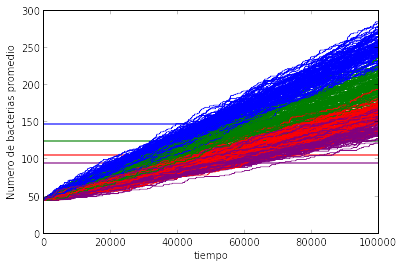
\includegraphics[width=0.6\textwidth]{todasLasCorridas.png}
\caption{Población de R.rhodnii transformada}
\FloatBarrier
\end{figure}
\FloatBarrier

Finalmente, nos sorprendimos al encontrar que los fitness encontrados mejoraban al instertarles el plásmido (\textit{E.Coli} y \textit{Salmonella} con \textit{R1} y \textit{R.Rhodnii} observando las poblaciones). Esto puede va de cierta manera en contra del sentido común que sería que estos fitness deberían ser menores a 1 ya que producir el anticuerpo tiene cierto costo energético. Aunque esto involucra resultados muy interesantes, la única manera de conocer dichos fitness es realizar un trabajo experimental.

\renewcommand\refname{\vskip -1cm}
\section{Referencias}
\nocite{*}

\bibliographystyle{apacite}
\bibliography{Zotero}









%[1]Bacterial symbiosis and paratransgenic control of vector-borne Chagas disease



\end{document}
%%%%%%%%%%%%%%% this is title page style%%%%%%%%%